\setauthor{AC}
\section{Gesamtarchitektur der Anwendung}
Die Gesamtarchitektur der Anwendung folgt einem klar getrennten Aufbau zwischen Benutzeroberfläche und serverseitiger Verarbeitung. Der Schwerpunkt meines Projektteils lag auf dem Frontend, das mit Angular als Single-Page-Application umgesetzt wurde. Das Frontend übernimmt die Darstellung der Inhalte, die Navigation zwischen den Ansichten sowie die Interaktion mit den Benutzern. Die eigentliche Datenverarbeitung erfolgt über bereitgestellte REST-Schnittstellen, die vom Frontend angesprochen werden. Durch diese Trennung konnte die Benutzeroberfläche unabhängig von der serverseitigen Implementierung entwickelt und erweitert werden.

\begin{figure}[h]
    \centering
    \setlength{\fboxsep}{8pt}
    \begin{tabular}{c c c}
        \fbox{\parbox{0.24\textwidth}{\centering\textbf{Frontend}\\Angular SPA\\Filmsuche\\Detailansicht\\Abo-Verwaltung}} &
        $\Longleftrightarrow$ &
        \fbox{\parbox{0.24\textwidth}{\centering\textbf{Backend}\\Quarkus REST API\\Services\\DTOs\\Persistenz}} \\
        \multicolumn{3}{c}{} \\
        \fbox{\parbox{0.24\textwidth}{\centering\textbf{Authentifizierung}\\Keycloak\\Login\\Token\\Rollen}} &
        $\Longleftrightarrow$ &
        \fbox{\parbox{0.24\textwidth}{\centering\textbf{Externe API}\\TMDB\\Filmdaten\\Providerdaten}} \\
        \multicolumn{3}{c}{} \\
        \multicolumn{3}{c}{\fbox{\parbox{0.28\textwidth}{\centering\textbf{Relationale Datenbank}\\Benutzer\\Provider\\Abonnements\\Historie}}}
    \end{tabular}
    \caption{Graphische Gesamtarchitektur der Anwendung}
    \label{fig:system_architecture}
\end{figure}

\section{Kommunikation zwischen Frontend und Backend}
Die Kommunikation zwischen Frontend und Backend erfolgt über HTTP-basierte REST-Aufrufe. Im Frontend wurden dafür eigene Angular-Services verwendet, um Daten strukturiert von den Schnittstellen zu laden und an die Komponenten weiterzugeben \cite{angular_forms}. Dieses Vorgehen hat den Vorteil, dass die Komponenten selbst möglichst wenig Logik für Datenzugriffe enthalten und sich stärker auf Darstellung und Interaktion konzentrieren können.

Im Projekt wurden insbesondere Services für Filmdaten, Providerdaten und die Authentifizierungsanbindung eingesetzt. Dadurch konnte die Anwendung Suchanfragen, Detailansichten und benutzerspezifische Inhalte in einer einheitlichen Struktur verarbeiten. Für das Frontend war dabei vor allem wichtig, dass externe Daten zuverlässig geladen, zwischengespeichert und in geeigneter Form in der Oberfläche dargestellt werden.

Bei benutzerspezifischen Daten reicht ein normaler HTTP-Aufruf jedoch nicht aus. Solche Daten können nur dann vom Backend geladen werden, wenn das Frontend ein gültiges Bearer-Token mitsendet. Dieses Token wird nach erfolgreicher Anmeldung über Keycloak bereitgestellt und bei geschützten Anfragen im Authorization-Header übertragen. Auf diese Weise kann das Backend prüfen, ob der Benutzer authentifiziert ist und Zugriff auf die angeforderten Daten besitzt \cite{keycloak_docs,keycloak_home}.

\setauthor{AC}
\section{API-Integration externer Movie-Datenbanken}
Ein wichtiger Bestandteil der Anwendung ist die Darstellung von Filminformationen und Streaming-Anbietern. Aus Sicht des Frontends bestand die Aufgabe darin, diese Informationen benutzerfreundlich aufzubereiten und in unterschiedlichen Ansichten darzustellen. Dazu gehören insbesondere die Filmübersicht, die Detailansicht einzelner Filme sowie die Anzeige verfügbarer Anbieter.

Die Filmdaten werden über bereitgestellte Schnittstellen geladen und in Angular-Komponenten eingebunden. Für die Benutzeroberfläche war dabei entscheidend, dass Suchergebnisse übersichtlich dargestellt, Detailinformationen verständlich aufbereitet und Navigationswechsel zwischen Listen- und Detailansicht flüssig umgesetzt werden. Da die Anwendung als Single-Page-Application realisiert wurde, konnte dieser Wechsel ohne vollständigen Seitenneuaufbau erfolgen \cite{mdn_spa}. Als externe Grundlage diente dabei die Dokumentation der TMDB API, insbesondere für Authentifizierung, Filmdaten und Anbieterinformationen \cite{tmdb_getting_started,tmdb_watch_providers}.

\begin{figure}[H]
    \centering
    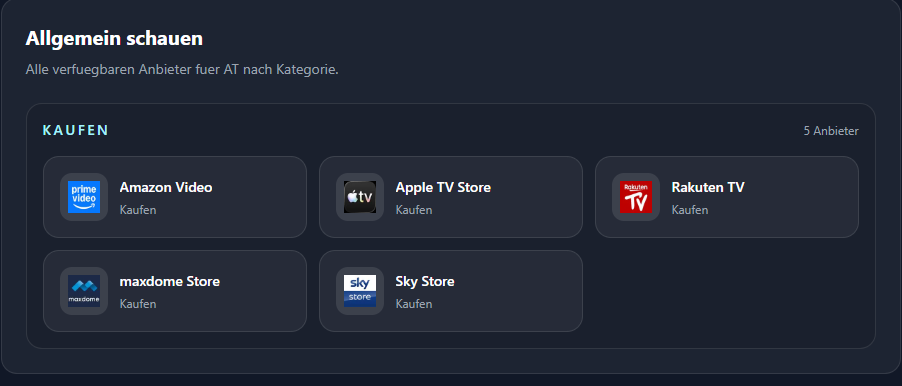
\includegraphics[width=\textwidth]{pics/Abbildung_2}
    \caption{Frontend-Ansicht der Anbieteranzeige innerhalb der Film-Detailansicht}
    \label{fig:placeholder_provider_view}
\end{figure}

\setauthor{AC}
\section{Sicherheits- und Datenschutzkonzept}
Aus Frontend-Sicht spielt das Sicherheits- und Datenschutzkonzept vor allem bei der Zugriffskontrolle auf geschützte Bereiche eine Rolle. Öffentliche Inhalte der Anwendung können ohne Anmeldung aufgerufen werden, während persönliche Funktionen wie die Verwaltung eigener Streaming-Abonnements nur nach erfolgreicher Authentifizierung zugänglich sind. Für diesen Zweck wurde Keycloak in das Frontend integriert \cite{keycloak_docs,keycloak_home}.

Ein wichtiger Bestandteil dieses Konzepts ist, dass personenbezogene oder benutzerspezifische Daten nicht öffentlich abrufbar sind. Das Backend stellt diese Informationen nur dann bereit, wenn bei der Anfrage ein gültiges Bearer-Token übertragen wird. Das Frontend übernimmt dabei die Aufgabe, den Authentifizierungsstatus zu verwalten und das Token bei geschützten Requests mitzuschicken. Dadurch wird sichergestellt, dass persönliche Inhalte nur autorisierten Benutzern angezeigt werden \cite{keycloak_docs}.

Die Angular-Anwendung erkennt den Authentifizierungsstatus der Benutzer und steuert darauf basierend den Zugriff auf geschützte Routen. Dadurch wird sichergestellt, dass sensible benutzerspezifische Inhalte nicht ohne Anmeldung angezeigt werden. Gleichzeitig verbessert diese Struktur die Benutzerfreundlichkeit, da sich öffentliche und persönliche Bereiche klar voneinander trennen lassen. Die eigentliche Verwaltung von Zugangsdaten erfolgt dabei nicht im Frontend selbst, sondern über das externe Authentifizierungssystem.
\input{./sections/datenbank}

\section{Backend-Architektur}
\setauthor{MT}

Die Backend-Architektur der vorliegenden Anwendung folgt einem mehrschichtigen Aufbau,
der eine klare Trennung der Verantwortlichkeiten gewährleistet. Dieses Architekturmuster
wird auch als \textit{Layered Architecture} bezeichnet. Jede Schicht übernimmt eine
klar definierte Aufgabe, wodurch die Wartbarkeit, Testbarkeit und Erweiterbarkeit
der Anwendung verbessert wird. Eine eingehende HTTP-Anfrage durchläuft dabei die
Resource-Schicht, wird über DTOs weitergeleitet, von der Service-Schicht verarbeitet
und schließlich über das Repository auf die Datenbankentitäten abgebildet.

\subsection{Entity}

Die Entity-Schicht repräsentiert die Datenmodelle einer Anwendung. Jede Entity-Klasse
bildet die Struktur einer Datenbanktabelle ab und wird mithilfe von Annotationen der
Jakarta Persistence API (JPA) mit der Datenbank verknüpft. Entity-Klassen enthalten
ausschließlich die Datenbankstruktur sowie einfache Zugriffsmethoden. Geschäftslogik
hat in dieser Schicht keine Berechtigung, da dies die Trennung der Verantwortlichkeiten
verletzen würde.

\subsection{Repository}

Die Repository-Schicht kapselt den Zugriff auf die Datenbank und stellt eine
Abstraktion zwischen der Datenzugriffslogik und den darüberliegenden Schichten dar.
Sie definiert die grundlegenden CRUD-Operationen (Create, Read, Update, Delete) sowie
komplexere Datenbankabfragen. Durch diese Trennung bleibt die Geschäftslogik
unabhängig von der konkreten Datenbankimplementierung, was einen späteren Austausch
der Persistenzschicht erleichtert und die Testbarkeit der Anwendung erhöht.

\subsection{Service}

Die Service-Schicht beinhaltet die Geschäftslogik der Anwendung und fungiert als
Vermittler zwischen der Resource- und der Repository-Schicht. Sie ist verantwortlich
für die Verarbeitung und Transformation von Daten, die Koordination mehrerer
Repository-Zugriffe sowie die Kommunikation mit externen Systemen. Die Service-Schicht
stellt sicher, dass die Geschäftsregeln der Anwendung zentral und unabhängig von
der Präsentations- oder Datenzugriffsschicht definiert sind.

\subsection{Resource}

Die Resource-Schicht ist für die Bereitstellung der RESTful-Endpunkte verantwortlich.
Sie nimmt eingehende HTTP-Anfragen entgegen, delegiert die Verarbeitung an die
zuständigen Service-Klassen und gibt die entsprechenden Antworten an den Client zurück.
Die Resource-Schicht enthält dabei selbst keine Geschäftslogik, sondern fungiert
ausschließlich als Schnittstelle zwischen dem Backend und den konsumierenden Clients.
Durch diese strikte Trennung bleibt die Schicht schlank und leicht austauschbar.

\subsection{DTO -- Data Transfer Objects}

Data Transfer Objects (DTOs) sind speziell zugeschnittene Datenobjekte, die dem
gezielten Datenaustausch zwischen verschiedenen Schichten oder zwischen Backend und
Client dienen. Anstatt vollständige Entity-Objekte direkt weiterzugeben, werden DTOs
verwendet, die ausschließlich jene Felder enthalten, die für den jeweiligen
Anwendungsfall erforderlich sind.

DTOs erfüllen dabei zwei wesentliche Zwecke. Erstens erhöhen sie die Sicherheit der
Anwendung: Sensible Felder einer Entity, wie etwa Passwort-Hashes oder interne
Systemfelder, werden nicht versehentlich nach außen weitergegeben. Zweitens wird
eine Entkopplung zwischen der internen Datenstruktur und der nach außen sichtbaren
API-Struktur erreicht. Änderungen am Datenbankmodell haben dadurch keinen direkten
Einfluss auf die API-Schnittstelle, was die Stabilität der Anwendung langfristig
sichert.


%----------------------------------------------------------
\section{Implementierung des Backends in der vorliegenden Applikation}
\setauthor{MT}

Die im vorherigen Abschnitt beschriebenen Architekturprinzipien wurden in der
vorliegenden Anwendung konsequent umgesetzt. Das Backend basiert auf Quarkus und
verwendet Hibernate ORM für die Datenbankanbindung. Die folgende Beschreibung
erläutert, wie die einzelnen Schichten konkret implementiert wurden.

\subsection{Entity}

Die Datenbankstruktur der Anwendung wird durch fünf Entity-Klassen sowie ein
Enum abgebildet, die gemeinsam das Domänenmodell der Anwendung repräsentieren.

Die zentrale Entität ist \texttt{UserMovieDB}, welche einen registrierten Benutzer
der Anwendung darstellt. Als Primärschlüssel wird dabei keine automatisch generierte
Datenbank-ID verwendet, sondern die \texttt{UUID} des Benutzers aus dem
Identity-Provider Keycloak. Dies stellt sicher, dass die interne
Benutzerrepräsentation direkt mit dem Authentifizierungssystem verknüpft ist.

Die Entität \texttt{Provider} repräsentiert einen Streaming-Anbieter wie etwa
Netflix oder Amazon Prime. Neben einer internen Datenbank-ID speichert sie die
\texttt{tmdbProviderId}, also die eindeutige ID des Anbieters in der TMDB API.
Diese dient als Brücke zwischen den intern gespeicherten Providern und den von
der externen API gelieferten Daten. Jedem Provider kann zusätzlich eine Liste
von \texttt{CountryPriority}-Einträgen zugeordnet werden, die die Anzeigepriorität
des Anbieters je nach Land abbilden.

Die Verknüpfung zwischen Benutzer und Streaming-Anbieter erfolgt über die
Entität \texttt{UserProviderSubscription}. Diese speichert neben den
Fremdschlüsseln auf \texttt{UserMovieDB} und \texttt{Provider} auch den
Abrechnungszyklus des Abonnements sowie das letzte Abrechnungsdatum. Der
Abrechnungszyklus wird über das Enum \texttt{BillingCycle} mit den
Ausprägungen \texttt{MONTHLY} und \texttt{YEARLY} abgebildet. Eine eindeutige
Kombination aus Benutzer und Anbieter wird durch eine
\texttt{UniqueConstraint}-Annotation auf Datenbankebene sichergestellt, sodass
ein Benutzer denselben Anbieter nicht mehrfach abonnieren kann. Die Entität
stellt zudem eine berechnete Methode \texttt{getNextBillingDate()} bereit, die
basierend auf dem Abrechnungszyklus das nächste Fälligkeitsdatum ermittelt.

Die Entität \texttt{History} speichert den Filmschauerverlauf eines Benutzers.
Sie referenziert den jeweiligen Benutzer über einen Fremdschlüssel sowie die
\texttt{tmdbMovieId} des gesehenen Films. Der Zeitpunkt des Ansehens wird
automatisch beim Erstellen eines \texttt{History}-Eintrags auf den aktuellen
Zeitstempel gesetzt.

\subsection{Repository}

Die Repository-Schicht der Anwendung besteht aus drei Klassen, die jeweils
den Datenbankzugriff für eine bestimmte Entität kapseln.

Das \texttt{UserMovieDBRepository} implementiert das \texttt{PanacheRepository}-
Interface und stellt spezialisierte Abfragemethoden bereit. Die Methode
\texttt{findByUUID} sucht einen Benutzer anhand seiner Keycloak-UUID und gibt
ein \texttt{Optional} zurück, um den Fall eines nicht vorhandenen Benutzers
typsicher zu behandeln. Die Methode \texttt{getUserProviderTmdbIds} liefert
alle TMDB-Provider-IDs der Abonnements eines bestimmten Benutzers als
\texttt{Set}, das anschließend im Service-Layer für den Abgleich mit der
TMDB API verwendet wird. Besonders hervorzuheben ist die Methode
\texttt{getProvidersWithOwnership}, die mithilfe einer JPQL-Abfrage alle
Provider aus der Datenbank lädt und dabei über einen \texttt{LEFT JOIN} mit
den Abonnements des Benutzers verknüpft. Das Ergebnis enthält für jeden
Provider ein Flag, das angibt, ob der Benutzer diesen abonniert hat. Dadurch
kann das Frontend mit einem einzigen Request alle relevanten Informationen
abrufen. Darüber hinaus enthält das Repository die Methode
\texttt{updateSubscriptions}, die die Abonnements eines Benutzers anhand
einer übergebenen Liste von \texttt{SubscriptionUpdateDTO}-Objekten
aktualisiert. Dabei werden neue Abonnements angelegt, bestehende
aktualisiert und nicht mehr enthaltene entfernt.

Das \texttt{ProviderRepository} verwaltet die Streaming-Anbieter in der
Datenbank. Die zentrale Methode ist \texttt{upsertFromTmdb}, die beim
Anwendungsstart aufgerufen wird: Sie prüft, ob ein Provider mit der
gegebenen \texttt{tmdbProviderId} bereits existiert, und aktualisiert
dessen Daten oder legt einen neuen Eintrag an. Dadurch wird eine konsistente
Synchronisierung der Provider-Daten mit der TMDB API gewährleistet.

Das \texttt{HistoryRepository} implementiert ebenfalls das
\texttt{PanacheRepository}-Interface und stellt Methoden für den Zugriff
auf den Filmschauerverlauf bereit. Die Methode \texttt{findByUserId} gibt
alle History-Einträge eines Benutzers sortiert nach dem Zeitpunkt des
Ansehens zurück. Über \texttt{findByUserIdLimit} kann die Anzahl der
zurückgegebenen Einträge begrenzt werden, was eine einfache Paginierung
ermöglicht. Die Methode \texttt{hasWatchedMovie} prüft, ob ein Benutzer
einen bestimmten Film bereits gesehen hat.

\subsection{Service}

Die Service-Schicht der Anwendung besteht aus drei Klassen, die jeweils
einen klar abgegrenzten Verantwortungsbereich abdecken.

Der \texttt{UserService} ist für die Verwaltung des aktuell authentifizierten
Benutzers zuständig. Er liest die Keycloak-UUID aus dem JWT-Token aus und
prüft über das \texttt{UserMovieDBRepository}, ob der Benutzer bereits in
der Datenbank existiert. Ist dies nicht der Fall, wird automatisch ein neuer
\texttt{UserMovieDB}-Eintrag angelegt. Dieses Muster wird als
\textit{Lazy User Creation} bezeichnet und stellt sicher, dass beim ersten
authentifizierten Zugriff eines neuen Benutzers automatisch ein
Datenbankprofil erstellt wird, ohne dass eine explizite Registrierung
erforderlich ist.

Der \texttt{TmdbService} kapselt die gesamte Kommunikation mit der externen
TMDB API. Die HTTP-Anfragen werden über die Bibliothek OkHttp durchgeführt,
die empfangenen JSON-Antworten mit Jackson geparst und auf DTOs abgebildet.
Der API-Schlüssel wird nicht im Quellcode hinterlegt, sondern über den
Quarkus-Konfigurationsmechanismus mittels \texttt{@ConfigProperty} injiziert,
was die Sicherheit der Anwendung erhöht. Der Service stellt Methoden zum
Abrufen von Filminformationen per ID oder Suchbegriff, zum Laden verfügbarer
Streaming-Anbieter sowie zum Abrufen trendender Filme bereit. Die Methode
\texttt{getFilteredProvidersForUser} kombiniert dabei externe API-Daten mit
internen Datenbankdaten: Sie ruft die verfügbaren Provider eines Films von
der TMDB API ab, gleicht diese mit den vom Benutzer abonnierten Anbietern
aus der Datenbank ab und setzt das Flag \texttt{ownedByUser} im
zurückgegebenen \texttt{ProviderInfoDTO}. Die Ergebnisliste wird abschließend
so sortiert, dass die vom Benutzer abonnierten Anbieter an erster Stelle
erscheinen.

Der \texttt{ProviderSyncService} wird beim Start der Anwendung automatisch
ausgeführt, indem er auf das Quarkus-Lifecycle-Event \texttt{StartupEvent}
reagiert. Er ruft über den \texttt{TmdbService} alle verfügbaren
Streaming-Anbieter von der TMDB API ab und synchronisiert diese über die
\texttt{upsertFromTmdb}-Methode des \texttt{ProviderRepository} in die
lokale Datenbank. Dadurch ist sichergestellt, dass die Anwendung stets eine
aktuelle Liste aller Provider vorhält, ohne dass ein manueller
Synchronisierungsschritt erforderlich ist. Der gesamte Vorgang wird in einer
Transaktion ausgeführt, was durch die \texttt{@Transactional}-Annotation
sichergestellt wird.

\subsection{Resource}

Die Resource-Schicht der Anwendung besteht aus drei produktiven
Resource-Klassen, die die REST-Endpunkte des Backends definieren.

Die \texttt{MovieResource} stellt Endpunkte unter dem Basispfad
\texttt{/api/movies} bereit. Sie ermöglicht das Abrufen von Filmdaten anhand
einer ID oder eines Suchbegriffs, das Laden verfügbarer Streaming-Anbieter
für einen Film sowie das Abrufen trendender Filme. Einige Endpunkte sind
öffentlich zugänglich und mit \texttt{@PermitAll} annotiert, während der
Endpunkt \texttt{/api/movies/\{id\}/providers/for-user} eine gültige
Authentifizierung erfordert und über \texttt{@RolesAllowed} auf die Rollen
\texttt{user} und \texttt{medien-abo-users-role} beschränkt ist. Bei diesem
Endpunkt wird die Benutzer-ID direkt aus dem JWT-Token extrahiert, sodass
keine User-ID in der URL übermittelt werden muss.

Die \texttt{UserResource} stellt Endpunkte unter dem Basispfad
\texttt{/api/users} bereit und ist vollständig authentifizierungsgeschützt.
Sie bietet Funktionalitäten zur Verwaltung des eigenen Benutzerprofils, der
Streaming-Abonnements sowie der Filmschauhistorie. Über
\texttt{GET /api/users/me} kann der aktuelle Benutzer seine Profildaten
abrufen, wobei bei einem erstmaligen Zugriff automatisch ein Datenbankprofil
angelegt wird. Der Endpunkt \texttt{PUT /api/users/me/subscriptions} ermöglicht das vollständige Aktualisieren der Abonnements in einem einzigen
Request. Die History-Endpunkte erlauben das Hinzufügen, Abrufen und Löschen
von Einträgen im Filmschauerverlauf. Beim Löschen wird explizit geprüft, ob
der Eintrag dem authentifizierten Benutzer gehört, bevor die Operation
ausgeführt wird.

Die \texttt{ProviderRessource} stellt Endpunkte unter \texttt{/api/providers}
bereit. Sie ermöglicht das Abrufen aller in der Datenbank gespeicherten
Streaming-Anbieter sowie das manuelle Auslösen einer Synchronisierung mit
der TMDB API über den Endpunkt \texttt{GET /api/providers/sync}.

\subsection{DTO -- Data Transfer Objects}

In der vorliegenden Anwendung werden DTOs konsequent eingesetzt, um die
Kommunikation zwischen den Schichten zu strukturieren und interne
Datenbankstrukturen zu kapseln.

Der \texttt{ProviderInfoDTO} wird bei der Abfrage von Streaming-Anbietern
eines Films verwendet. Er enthält die TMDB-Provider-ID, den Anbieternamen,
die URL des Provider-Logos sowie das Flag \texttt{ownedByUser}, das angibt,
ob der jeweilige Benutzer diesen Anbieter abonniert hat. Die vollständige
\texttt{Provider}-Entity sowie interne Datenbankfelder werden dabei nicht
weitergegeben.

Der \texttt{ProviderWithOwnership}-DTO wird vom \texttt{UserMovieDBRepository}
direkt über eine JPQL-Konstruktorabfrage befüllt und an den Client
übermittelt. Er enthält neben den Provider-Stammdaten auch den
Abrechnungszyklus und das letzte Abrechnungsdatum des Abonnements, sofern
der Benutzer den jeweiligen Anbieter abonniert hat.

Der \texttt{SubscriptionUpdateDTO} dient als Eingabe-DTO für den
\texttt{PUT /api/users/me/subscriptions}-Endpunkt. Er enthält die
TMDB-Provider-ID, den gewünschten Abrechnungszyklus sowie das
Abrechnungsdatum und ermöglicht so die vollständige Aktualisierung eines
Abonnements in einem einzigen Objekt.

Der \texttt{TrendingMovieDTO} bündelt alle relevanten Informationen eines
trendenden Films -- Titel, Poster-URL, Kurzbeschreibung, Erscheinungsdatum,
Popularitätswert sowie Bewertungsdurchschnitt und Bewertungsanzahl -- in
einem kompakten Objekt, das direkt an den Client übermittelt wird.

Der \texttt{HistoryDTO} dient der strukturierten Rückgabe von
History-Einträgen an den Client. Er wird über eine statische
\texttt{from(History)}-Methode aus der gleichnamigen Entity erstellt und
stellt sicher, dass keine internen JPA-Proxies oder lazy-geladenen
Assoziationen versehentlich serialisiert werden.

Der \texttt{ProviderApi}-Record dient als internes Transferobjekt zwischen
dem \texttt{TmdbService} und dem \texttt{ProviderSyncService}. Er bildet
die Struktur der TMDB-API-Antwort ab und ermöglicht eine typsichere
Weiterverarbeitung der Rohdaten, bevor diese in die Datenbank geschrieben
werden.


